\subsection{LSTM}
\subsubsection{Overview of LSTM}
LSTM is a sophisticated architecture within Recurrent Neural Networks (RNNs), designed to address the limitations of traditional RNNs in capturing long-range dependencies in sequential data, 
a challenge often compounded by the vanishing gradient problem. The hidden layer of an LSTM consists of memory cells interconnected through a series of gates: the input gate, forget gate, and output gate, which collectively facilitate short-term memory storage.

\begin{enumerate}
	\item Forget gate:	The forget gate determines which information from the previous state should be discarded or retained. Mathematically, it is represented as:
	\begin{align}
		f_{t} &= \sigma(W_{f}x_{t} + U_{f}h_{t-1} + b_{f})
	\end{align}
	where $f_{t}$ is the output of the forget gate layer at the time step $t$, $W_{f}$, $U_{f}$, $b_{f}$ are the weight matrices and bias vectors for the forget gate computation, respectively.

	\item The input gate decides what new information should be stored in the cell. It operates as follows:
	\begin{align}
		i_{t} &= \sigma(W_{i}x_{t} + U_{i}h_{t-1} + b_{i}) \\
		g_{t} &= tanh(W_{c}x_{t} + U_{c}h_{t-1} + b_{c}) 
	\end{align}
	where $i_{t}$ is the output of the input gate layer at the time step $t$, $g_{t}$ is the candidate value to be added to the output layer at the time step $t$, $W_{i}$, $W_{c}$, $U_{i}$, $U_{c}$, $b_{i}$, $b_{c}$ are the weight matrices and bias vectors for the input gate and candiate value computation, respectively.
	
	\item The output gate determines which information from the cell should be used to generate the output. It is defined by:
	\begin{align}
		o_{t} &= \sigma(W_{o}x_{t} + U_{o}h_{t-1} + b_{o}) \\
		c_{t} &= f_{t} \odot c_{t-1} + i_{t} \odot g_{t} \\
		h_{t} &= o_{t} \odot tanh(c_{t})
	\end{align}
	where $o_{t}$ is the output of the output gate layer at the time step $t$, $c_{t}$ is the status of the cell at the time step $t$, $h_{t}$ is the output of the LSTM unit at the time step $t$, $W_{o}$, $U_{o}$, $b_{o}$ are the weight matrices and bias vectors for the output gate computation, respectively.
\end{enumerate}
Compared to the traditional RNN, LSTM performs various mathematical operations, including including element-wise multiplication and addition, to control the flow of information and perform updates to the memory cell and hidden state.

Compared to traditional RNNs, LSTMs perform a variety of mathematical operations, including element-wise multiplication and addition, to control the flow of information and update the memory cell and hidden state. 
This architecture enables LSTMs to effectively handle long sequential data, making them capable of capturing time-dependent patterns in the data.

\subsubsection{Background of employing LSTM}

Stock prices are typically regarded as time series data, characterized by their sequential nature and the presence of temporal dependencies. 
LSTM is particularly well-suited for modeling such data due to their ability to capture both short-term and long-term dependencies and patterns. 
This capability stems from their unique architecture, which allows them to remember information over extended periods and forget irrelevant data, a critical feature for analyzing the often volatile and non-linear patterns observed in stock market data.

\subsection{GRU}
\subsubsection{Overview of GRU}

GRU is a type of RNN architecture, offering a simpler alternative to LSTM. 
Despite their simpler structure, GRUs have proven highly effective in various applications. They are designed to address the vanishing gradient problem, enabling RNNs to better capture long-range dependencies in sequential data. 
A distinctive feature of GRUs, as compared to LSTMs, is their unified approach to managing cell state and output, which simplifies the architecture.

GRUs utilize two main gates for their operation:
\begin{enumerate}
	\item Update gate: 	The update gate determines how much of the past information needs to be passed along to the future.
	\begin{equation}
		z_{t} = \sigma(W_{z}x_{t} + U_{z}h_{t-1} + b_{z})
	\end{equation}
	\item Reset gate:	The reset gate decides how much of the past information to forget.
	\begin{align}
		r_{t} &= \sigma(W_{r}x_{t} + U_{r}h_{t-1} + b_{r})
	\end{align}
\end{enumerate}
These gates help the GRU to make decisions about what information is relevant to keep from past time steps and what can be discarded, 
enabling it to capture dependencies over different time scales effectively.


\subsubsection{Background of employing GRU}

Similar to LSTMs, GRUs are employed with the expectation that they can capture both short-term and long-term dependencies and patterns in sequential data. 
GRU, with their simplified structure, offers an efficient way to model these complexities.

\subsection{Transformer}

The Transformer is a neural network architecture that has revolutionized the field of natural language processing (NLP) and has shown promising potential in time series prediction tasks. 
Unlike traditional RNN-based models like LSTM and GRU, the Transformer relies entirely on an attention mechanism.
% \begin{wrapfigure}{r}{0.4\textwidth}
% 	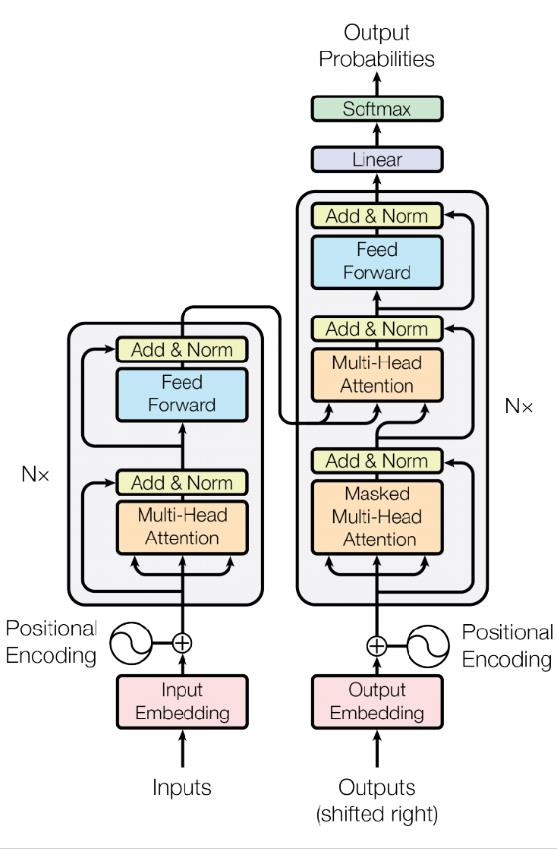
\includegraphics[width=0.4\textwidth]{Fig/Transformer.jpg}
% 	\caption{Transformer model structure}
% \end{wrapfigure}
\subsubsection{Overview of Transformer}
Transformer operates as an Encoder-Decoder model, leveraging an attention mechanism.
In the Encoder-Decoder architecture, the Encoder takes an input sequence and encodes the information into a single context vector. 
Conversely, the Decoder utilizes this context vector to generate an output sequence.
Within the model structure, a crucial component is the "embedding" process. 
This process involves the conversion of input values into a unified vector representation.

The attention mechanism employed by the Transformer is a key feature. 
It assigns varying weights to elements within the input sequence, placing greater emphasis on pertinent information. 
This emphasis is then reflected in the model's output. 
The Transformer employs this mechanism to comprehensively evaluate the significance of the entire input sequence when generating the output.

\subsubsection{Background of employing Transformer}

The decision to employ the Transformer model in stock price prediction stems from its advanced capabilities in handling sequential data. 
While LSTM and GRU have made significant strides in addressing the vanishing gradient problem, they still have limitations, particularly in their sequential processing nature and in fully capturing long-range dependencies.
The expectation is that the Transformer, with its advanced architecture, will outperform traditional models like LSTM and GRU in capturing the intricate patterns and dependencies inherent in stock price data, leading to more accurate and reliable predictions.

\subsection{Loss function}
\begin{figure}
	\centering
	
\includegraphics[width=0.8\textwidth]{Fig/loss_function.png}
	\caption{Huber loss function}
	\label{fig:huber_loss}
\end{figure}

\subsubsection{Overview of Loss function}
In our model, the loss function is defined as:
\begin{equation}
	\mathcal{L} = \mathcal{L}_{H} + \lambda \sqrt{\sum \left( \frac{\hat{y}_{t} - {y}_{t}}{{y}_{t-1} - {y}_{t}} \right)^{2}}
\end{equation}
where $\mathcal{L}_{H}$ is Huber loss function, $\lambda$ is a regularization parameter, $y_{t}$ is the actual value at time step $t$, and $\hat{y}_{t}$ is the predicted value at time step $t$.
The Huber loss function is given by:
\begin{equation}
	\label{eq:huber_loss}
	\mathcal{L}_{H} = \sum_{t=1}^{n} \begin{cases}
		\frac{1}{2}(y_{t} - \hat{y}_{t})^{2} & \text{tf } |y_{t} - \hat{y}_{t}| \leq \delta \\
		\delta |y_{t} - \hat{y}_{t}| - \frac{1}{2}\delta^{2} & \text{otherwise}
	\end{cases}
\end{equation}

The Huber loss function is chosen for its balanced approach, combining the robustness of the L1 norm with the smoothness of the L2 norm. 
This makes it differentiable and less sensitive to outliers in the data. 
Visually, the Huber loss resembles the L2 norm for smaller errors but transitions to an L1 norm-like behavior for larger errors, effectively handling outliers as seen in the Figure \ref{fig:huber_loss}.

Additionally, we incorporated a regularization term into the loss function. 
This term is designed to provide some leniency for rapid changes in stock prices. 
It implies that the model is less penalized for missing rapid price changes, acknowledging the inherent volatility and unpredictability in stock price movements.


\subsubsection{Background of employing Loss function}

Initially, our model employed the Huber loss function without a regularization term. 
However, we observed that the model tended to predict the next day's stock price as being equal to the current day's price, a pattern inconsistent with real-world stock market behavior. 
This phenomenon aligns with the martingale theory in probability, where the expected next value of a sequence of random variables is simply the current value.

Recognizing that stock prices are not merely a sequence of random variables but are influenced by trends and patterns, we introduced the regularization term. 
This addition encourages the model to recognize and respond to short-term trends in stock prices, rather than strictly adhering to the immediate past value. 
It allows the model to be more responsive to rapid changes, aligning its predictions more closely with the dynamic nature of the stock market.


\subsection{VADER}

\subsubsection{Overview of VADER}
VADER (Valence Aware Dictionary and sEntiment Reasoner) is a rule-based model specifically designed for sentiment analysis of social media text. 
It excels in analyzing the sentiment of individual words and phrases, providing an overall sentiment score for the text. 
VADER employs a combination of lexical elements and grammatical heuristics to assess sentiment, effectively capturing both the polarity (positive or negative) and intensity of emotions expressed in the text.

One of VADER's strengths lies in its ability to adeptly handle the unique characteristics of social media text, such as slang, emoticons, and abbreviations, which are often challenging for traditional sentiment analysis models. 
Its performance in sentiment analysis tasks, especially in the context of social media, is notably high. 

\subsubsection{Background of employing VADER}

In our stock price prediction model, we integrated VADER to incorporate additional factors that could influence stock prices. 
While our model effectively captures short-term trends in stock prices—predicting rises or falls based on recent price movements—it sometimes struggles to anticipate when these trends might not hold.

To address this, we turned to external factors like news, which can significantly impact stock prices both in the short and long term. 
News sentiment, whether positive or negative, along with the intensity of the sentiment, can be pivotal in shaping stock market trends. 
VADER's ability to evaluate these sentiments provides a nuanced understanding of how news might affect stock prices.

We use VADER to generate sentiment scores for news articles, incorporating these scores as new factors in our model. 
This approach aims to enhance the model's predictive accuracy by accounting for the influence of news sentiment on stock price movements, capturing new trends that might not be evident from historical price data alone.
